

\subsection{Dataset}

We use three datasets in our study. 
All of the datasets are collected by a gradually 
improved Android app.  
There are totally more than 13,000 miles of driving data 
collected in both controlled and uncontrolled environments
over the past three years.  
We will make our dateset available to public after 
this work has been published.  


\textbf{Dataset $\#1$}. 
We deploy Xoom tablets installed with our app on 10 different cars. 
The tablets collect the vehicular speed data from the On-board diagnostics (OBD)
port and various sensor data (including GPS and inertial sensors).  
Each tablet is placed in the back pocket of the passenger seat. 
The invovled cars are from different models and the stability
of the tablet placement is different, 
which provides the opportunity to study the effects of 
mounting stability on motion estimation accuracy.   


\textbf{Dataset $\#2$}.
We also collect some data in more controlled environments, 
where we know what is happening and the groundtruth data are recorded. 
First, we collect the data when the smartphone is placed in various scenarios, 
i.e., holding by hand, fixed by car mount holder, placed in cup holder etc. 
These data are used to understand various orientations and 
the relation between mounting stability and motion estimation accuracy.  
Second, we collect some data when randomly changing the 
orientation of the smartphone, i.e., 
move the smartphone from pocket and fix it on car mount holder. 
These data are used to evaluate the accuracy of 
our orientation change detection module. 
Third, we collect some data from two devices, where one device
is manually aligned with the car (as best as we can), 
and the other is fixed in car mount holder or held in passenger's hand. 
These data are used in two cases. 
One trip is used to understand acceleration
overestimation problem caused by gravitational force. 
Another 10 trips are used to estimate the
vehicle steering motions, where the gyroscope readings 
of manually aligned device is used as groundtruth data. 
 

\textbf{Dataset $\#3$}. 
We release the beta version of the Android app 
to 9 volunteers. 
The trip recording module is written as an Android Service,
so it is running in the background while the user may use 
the smartphone for navigation, game or any other activities. 
These data are used to understand how different users
are placing their smartphones while driving or 
sitting in the car. 



\subsubsection{Road Slope Statistics}

\begin{figure}[ht]
\begin{center}
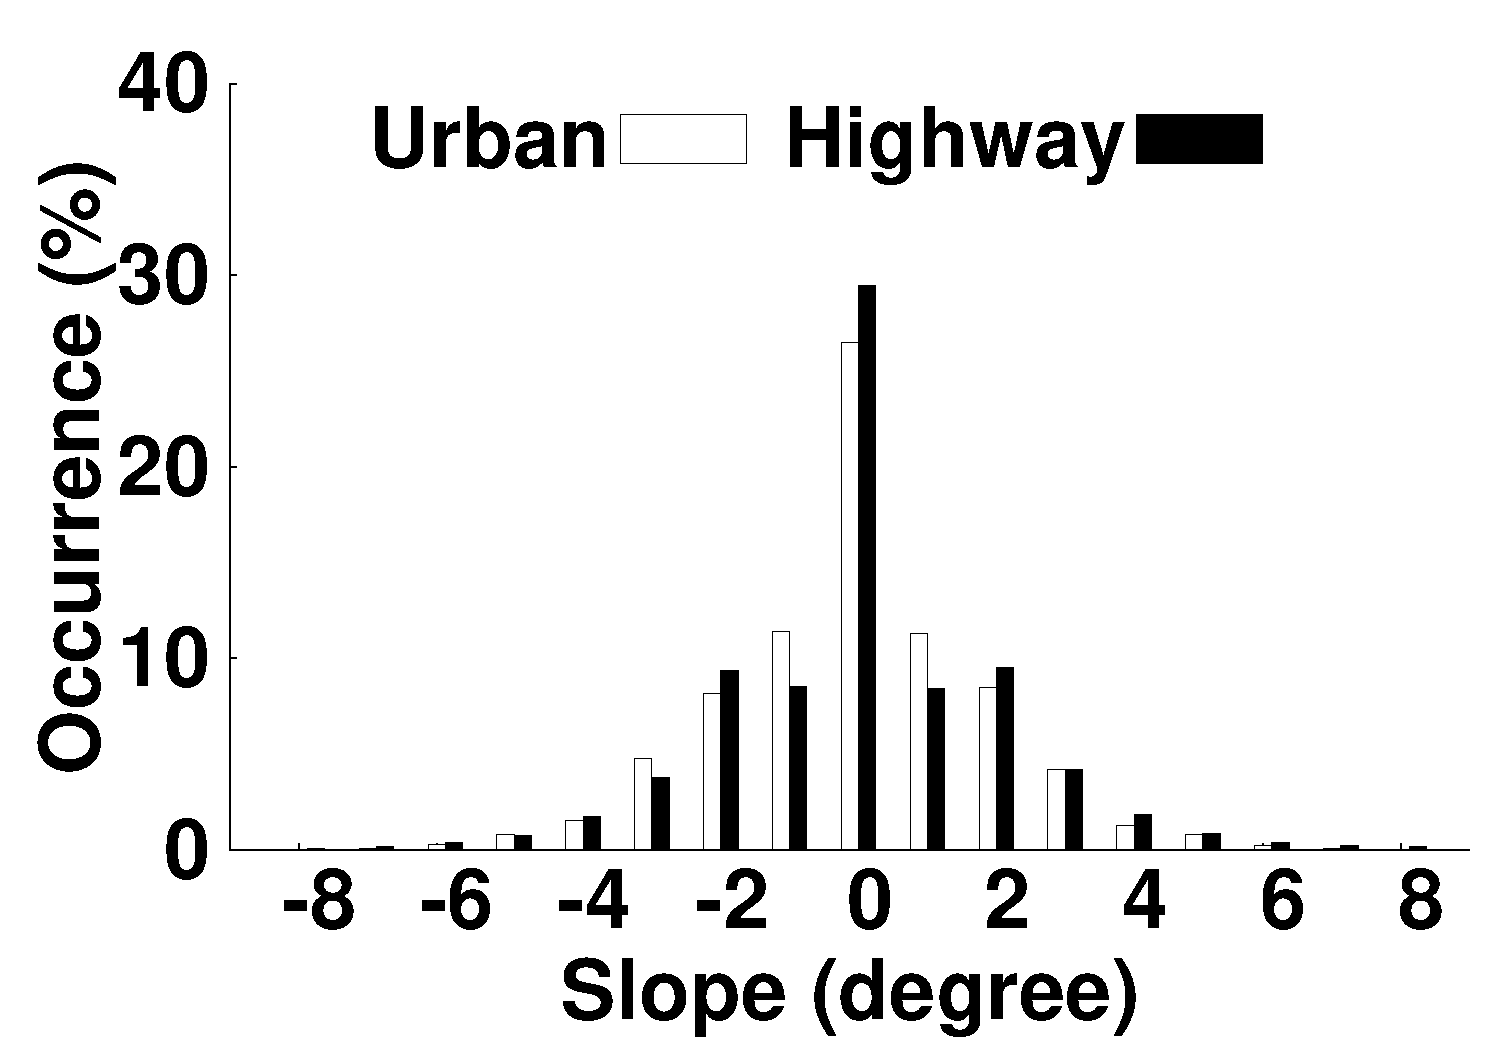
\includegraphics[width=3.5in, angle=0]{Figs/DriveSense/slopeaware/degrees.pdf}
\caption{Histogram of slope gradients. The acceleration estimation error is 
proportional to $gsin\theta$, where $\theta$ is the road slope angle.}
\label{slopegradients}
\vspace{-0.4cm}
\end{center}
\end{figure}


As we discussed above, the slopes introduce linear acceleration estimation errors.
An important question is how many road segments are sloping and
how many of them are actually level. 
Some cities, e.g., San Diego and Los Angeles, are full of hills, 
and most roads are sloping roads.
Surprisingly, in a plain area in US where we collect data, 
there are also full of slopes. 
To obtain the road gradient, we use the Google elevation dataset \cite{googleelevation}. 
For each GPS data point, we queried the elevation from the dataset. 
and calculated the gradient by the elevation difference
and distance.
We eliminated the close consecutive GPS data points that less than 5 meters in distance and removed the data points where the speed is less than $10mph$.
As we can see from the histogram in Fig. \ref{slopegradients}, 
more than half of the roads are not flat.
Those sloping roads, even as small as two degrees, may introduce accumulated
errors on coordinate alignment and further slope estimation, i.e., $0.34m/s^2$.
The aggregated error may cause significant linear acceleration estimation error
and introduce false positives/negatives on brake/acceleration monitoring. 




\subsection{Improved Overall Accuracy}

\subsubsection{Acceleration Estimation}


We use dataset $\#1$ to evaluate the accuracy of DriveSense and
other methods. 
The other three methods are using Accelerometer with Traditional Coordinate
Alignment (TCA)  \cite{hansenspeed, wang2013sensing, chen2015invisible}, 
Slope-Aware coordinate alignment with linear 
acceleration estimation, 
and GPS.
In this evaluation, we only use the tight group data where the 
tablet is stably fixed in the car.  
Therefore, the results generated by sensors are 
the best cases can be achieved for sensor-based motion estimations. 
We compare the acceleration difference between
each method and the groudtruth (calculated by OBD speed). 
The results are shown in Fig. \ref{xsense_accuracy}. 
The estimation made by well-tuned sensor coordinate alignment and 
linear acceleration estimation (Slope-Aware curve)
shows similar $80\%$ accuracy with GPS. 
The gap between Slope-Aware and Accelerometer are caused
by road slopes, 
where slope-unaware solution will over/under-estimate 
acceleration due to gravitational force. 
The accuracy gain of DriveSense is from the 
acceleration estimation compensation by sensors
when the GPS speed is low. 

 

\begin{figure}[th]
\begin{center}
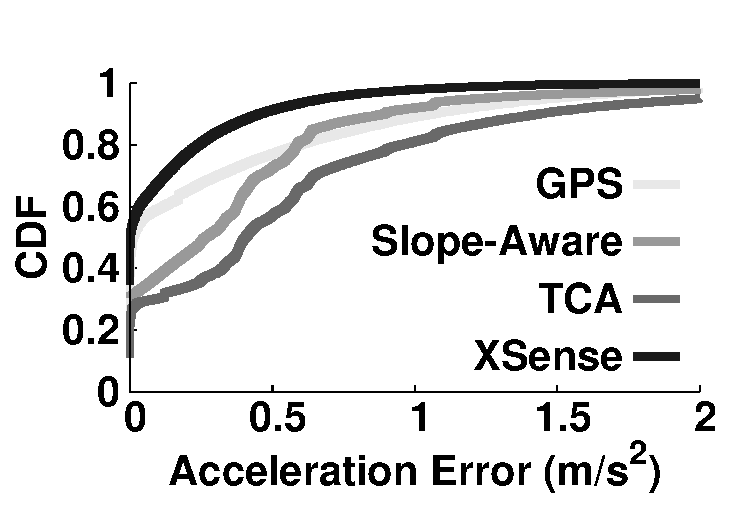
\includegraphics[width=3.0in,angle=0]{Figs/DriveSense/evaluation/xsense_accuracy.pdf}
\vspace{-0.2cm}
\caption{Comparing acceleration estimation accuracy among various methods.}
\vspace{-0.3cm}
\label{xsense_accuracy}
\end{center}
\end{figure}





\subsubsection{Steering Angular Velocity Estimation}


\begin{figure}[!htbp]
\begin{center}
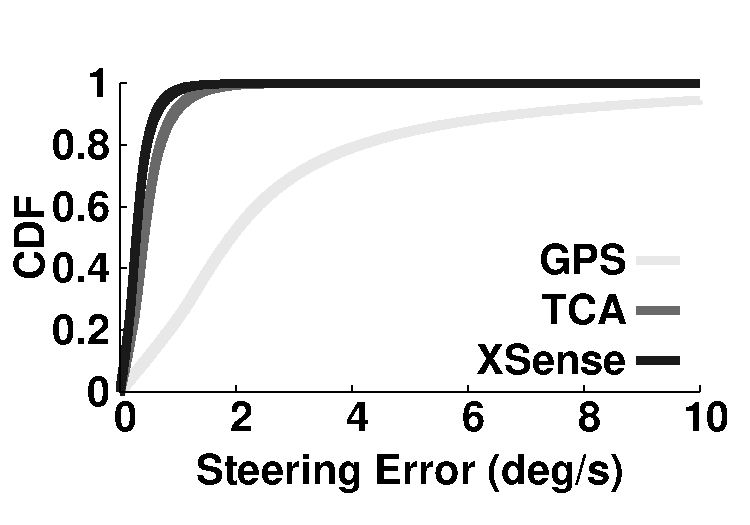
\includegraphics[width=3.0in,angle=0]{Figs/DriveSense/evaluation/evaluation_steering.pdf}
\vspace{-0.2cm}
\caption{Comparing steering angular velocity estimation accuracy among various methods. }
\vspace{-0.3cm}
\label{xsense_steering}
\end{center}
\end{figure}

We use dataset $\#2$ to evaluate steering angular velocity 
estimations. 
In this setting, one device is manually aligned with
the car and the gyroscope reading of which is used
as the groundtruth. 
Another device is fixed in car mount holder.    
As expected and can be seen in Fig. \ref{xsense_steering}, 
GPS can not estimate angular velocity accurate enough
for small horizontal movement such as lane change due to
its large estimation errors. 
DriveSense performs slightly better than gyroscope with 
Traditional Coordinate Alignment (TCA) due to 
the slope-aware solution presented in this work. 
The gain is obtained in the cases where the coordinate
alignment is conducted on slope, and there is vertical
misalignment caused by slope-unaware coordinate alignment. 




\subsection{Orientation Change Detection}

We evaluate the orientation change module
by using dataset $\#2$ in this section. 


\textbf{Detection Rate}.
The performance of inertial sensors in vehicle
motion sensing applications highly depends
on the fixed relative orientation between
the smartphone and the car. 
Therefore, detecting orientation change is 
very important in such applications. 
We evaluate the orientation change detection methods 
in two settings, tight setting and loose setting. 
In tight setting, the smartphone is mounted in 
various orientations on the car mount holder, 
or mounted by car cup holder. 
In loose setting, the smartphone is put in 
pocket, placed in passenger seat, or holding by 
passenger's hand. 
For each orientation, we record 
the groundtruth by a customized app. 
We use more than 10 trips and record
98 orientation changes in tight setting 
and 82 orientation changes in loose setting. 
The detection rate is presented in Table \ref{evaluate_change}. 
The Moving Variance method can detect most
of the orientation changes expect when 
there is small horizontal orientation change. 
But such orientation change will increase the 
Intra-Cluster Variance so that the stability 
detection module can identify
the polluted sensor output. 


\begin{table}[ht]
        \vspace{0.5cm}
        \centering
        \caption[evaluate_change]{Orientation Change Detection Accuracy}
         \vspace{0.0cm}
        \label{evaluate_change}
                \begin{tabular}{|l|c|c|}
                \hline
Method & Tight & Loose
\\  \hline      \hline
MV & $96.9\%$  &  $87.8\%$ 
\\  \hline
MV + ICV & $100\%$ & $96.3\%$   
\\  \hline
     \end{tabular}
\end{table}


%98 orientation changes
%95 detected with both
 
%82 loose orientaiton changes
%72 detected



\begin{figure}[!htbp]
\begin{center}
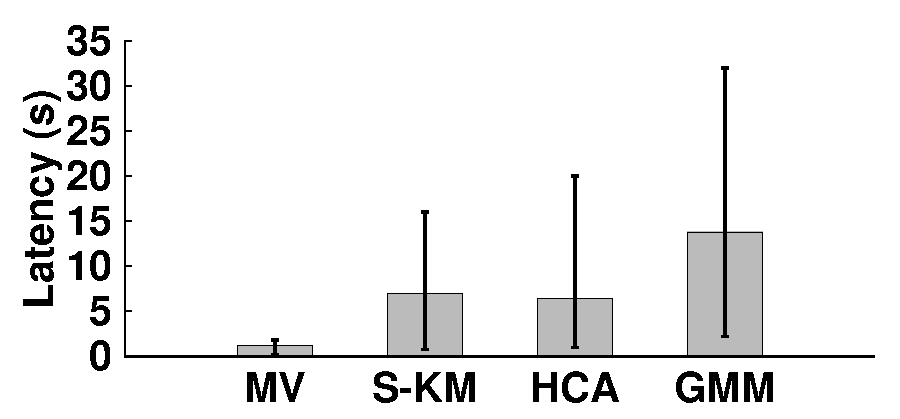
\includegraphics[width=3.0in,angle=0]{Figs/DriveSense/clustering_methods.pdf}
\vspace{0.0cm}
\caption{The time used to detect there is an orientation change.}
\vspace{-0.2cm}
\label{evaluate_latency}
\end{center}
\end{figure}


\textbf{Detection Latency}. 
Detecting orientation change timely can reduce possible inaccurate 
estimations. 
We compare the moving variance (MV) method with other common
data stream clustering method such as 
sequential K-means (SK), hierarchical clustering (HCA) 
and Gaussian Mixture Models (GMM). 
We run the four methods in 10 different orientation changes, 
and the results are shown in Fig. \ref{evaluate_latency}. 
MV can detect orientation change in 10-20 data samples (1-2s). 
The common incremental clustering techniques require more
time as it needs more data to form/detect another cluster. 



\subsection{Comparison Between GPS and IMU Sensors}

\begin{figure}[!htbp]
\begin{center}
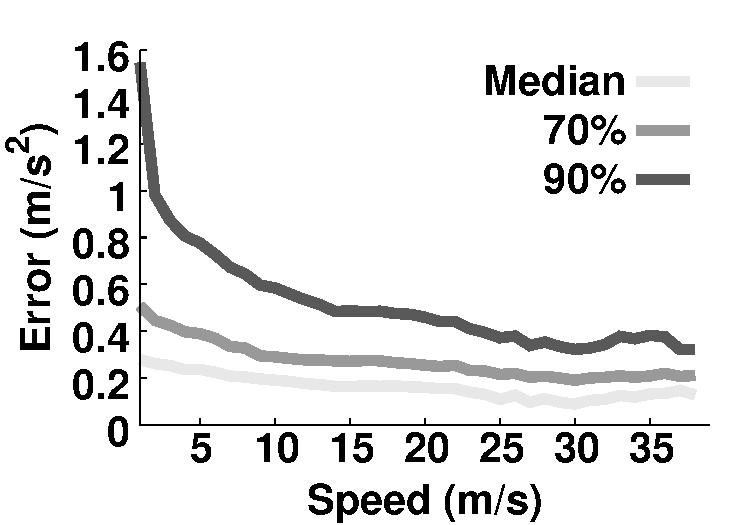
\includegraphics[width=3.0in, angle=0]{Figs/DriveSense/speed_acce_error.pdf}
\vspace{-0.2cm}
\caption{GPS acceleration estimation errors under various speeds.}
\vspace{-0.4cm}
\label{speed_acce_error}
\end{center}
\end{figure}




\begin{table}[!htbp]
        \centering
        \vspace{0.5cm}
        \caption[icv_accuracy]{Median ICV and Acceleration Estimation Accuracy}
         \vspace{0.0cm}
        \label{icv_accuracy}
                \begin{tabular}{|l|c|c|c|}
                \hline
ICV Median & Median Error & $70th-\%$ & $90th-\%$ 
\\  \hline      \hline
0.05 & $0.15m/s^2$  & $0.18m/s^2$ & $0.31m/s^2$ 
\\  \hline
0.21 & $0.21m/s^2$  &  $0.38m/s^2$ & $0.95m/s^2$   
\\  \hline
0.87 & $0.45m/s^2$ & $0.78m/s^2$ & $1.56m/s^2$   
\\  \hline
\end{tabular}
\end{table}


To select between IMU sensor and GPS as input
for acceleration estimation, 
we compare the accuracy based on current speed and 
mounting stability. 
To estimate the accuracy of GPS, 
we use one pipeline to process GPS stream data 
and track the speeds. 
Each GPS point is associated with a confidence value. 
The confidence value is the $\beta$$th$ percentile
estimation accuracy under given speed.
The percentile accuracy under various speeds
is illustrated in Fig. \ref{speed_acce_error}.
To estimate the accuracy of IMU sensors, 
we use ICV to track the mounting stability of the smartphone. 
We use the median ICV as an indicator of
the mounting stability. 
The corresponding percentile errors of different
ICV are illustrated in Table \ref{icv_accuracy}.



\subsection{Training Time}

\begin{figure}[!htbp]
\begin{center}
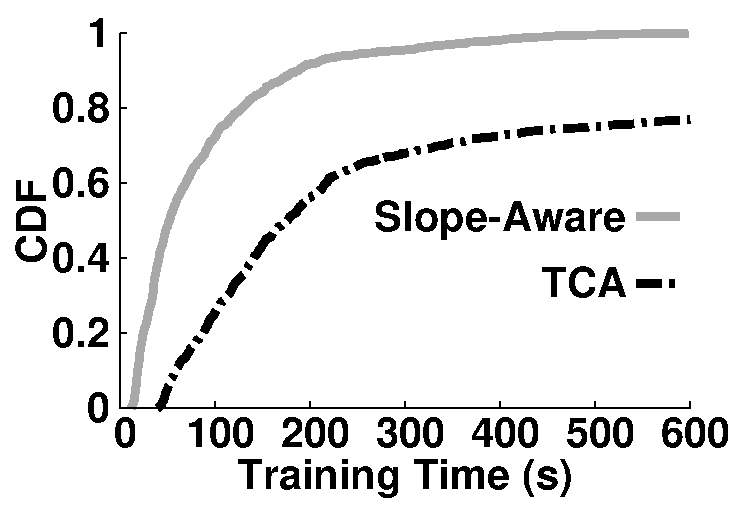
\includegraphics[width=2.8in,angle=0]{Figs/DriveSense/slopeaware/alignment.pdf}
\vspace{-0.2cm}
\caption{The training time used for coordinate alignment.}
\label{alignmenttime}
\vspace{-0.3cm}
\end{center}
\end{figure}

The training time of a coordinate alignment algorithm is critical
for real-time applications such as hard brake warning \cite{snapshot}. 
To evaluate the training time, we extract the straight road driving segments and fed them into the replay engine.
The engine stops when the accuracy of coordinate alignment is within
a predefined percentage of the accuracy when we use the segments of the entire trip to train.
As shown in Fig. \ref{alignmenttime}, 
there is a substantial improvement on the training speed.
Slope-aware alignment matrix can be trained in less than $2min$ in more than
$80\%$ of the cases, 
while it takes much longer time to train the rotation matrix if
the algorithm does not consider slope caused deviations.
The training time heavily depends on road conditions. 
For the trips with level roads and fewer bumps, it generally
takes less time to train.
On the other hand, for the trips with lots of slopes and bumps on the road, 
it takes much longer time to train due to less training opportunities.


\subsection{In the Wild}


%\subsubsection{Statistics}

\begin{figure}[!htbp]
\begin{center}
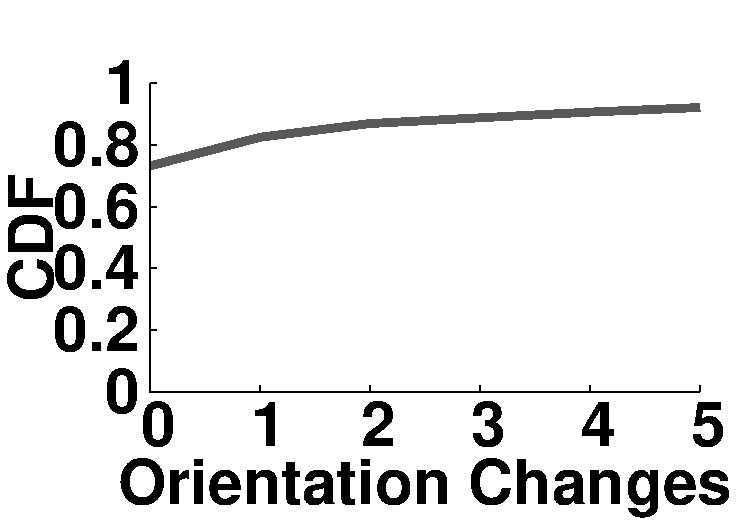
\includegraphics[width=1.7in,angle=0]{Figs/DriveSense/evaluation/wild_changes.pdf}
\hspace{-0.5cm}
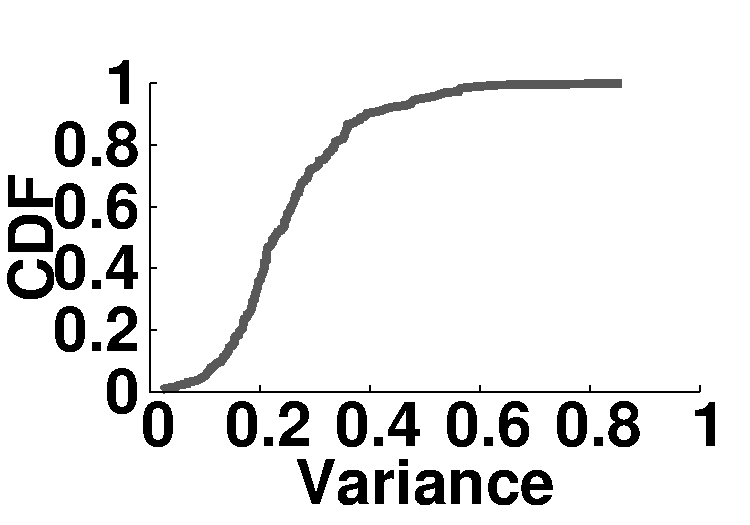
\includegraphics[width=1.7in,angle=0]{Figs/DriveSense/evaluation/wild_variances.pdf}
\vspace{0.0cm}
\caption{The orientation change and stability measurement statistics.}
\vspace{-0.2cm}
\label{wild_evaluation}
\end{center}
\end{figure}


The beta version of our Android application (the full version with 
trip upload, user management and back-end server etc.) is released to
9 volunteers for the past half year. 
There are totally 269 trips collected. 
The trip recording functionality of the app is designed as an Android 
Service, so it is able to run in the background. 
We observe some users forget to stop the app, 
so we add another functionality to stop recording if there
is no high speed movement in 10 minutes. 
The volunteers are asked to place the Android phone
at anywhere they prefer. 
Among the 269 trips we collected, 
orientation change occurs in 74 trips. 
The CDF of the orientation change statistics are 
illustrated in Fig. \ref{wild_evaluation}.
Normally it takes about several minutes to find a fragment
to train the rotation matrix, frequent changing 
the orientation may reduce the opportunities using
inertial sensors. 
We also evaluate the stability or the variance of the trips 
without orientation changes. 
The results, as shown in Fig. \ref{wild_evaluation}, 
indicate that the smartphones are mounted tightly
in most of cases. 
There are about $25\%$ trips where the smartphone is not 
tight enough (high variances) and GPS should be used instead. 


\nop{
\subsubsection{Parameter Selection}

\begin{figure}[!htbp]
\begin{center}
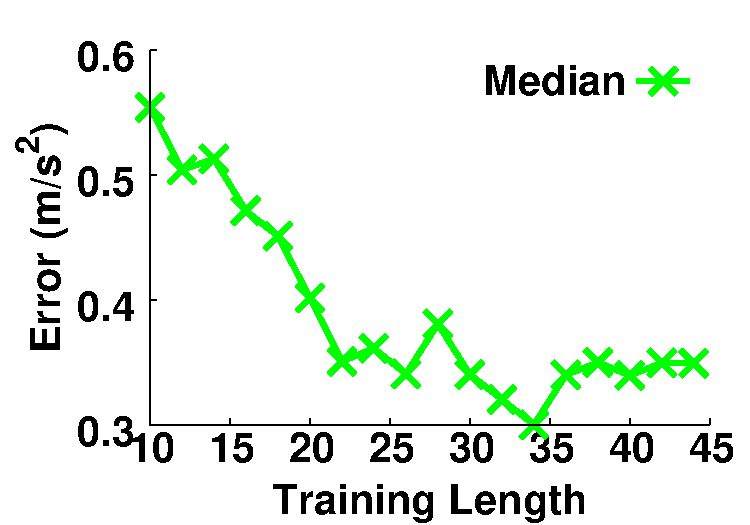
\includegraphics[width=1.7in,angle=0]{Figs/DriveSense/trainlengthanderror.pdf}
\vspace{0.0cm}
	\caption{The training length is related to horizontal alignment median error.}
\label{training}
\vspace{-0.2cm}
\end{center}
\end{figure}
}




